%%%%%%%%%%%%%%%%%%%%%%%%%%%%%%%%%%%%%%%%%
% Short Sectioned Assignment
% LaTeX Template
% Version 1.0 (5/5/12)
%
% This template has been downloaded from:
% http://www.LaTeXTemplates.com
%
% Original author:
% Frits Wenneker (http://www.howtotex.com)
%
% License:
% CC BY-NC-SA 3.0 (http://creativecommons.org/licenses/by-nc-sa/3.0/)
%
%%%%%%%%%%%%%%%%%%%%%%%%%%%%%%%%%%%%%%%%%

%----------------------------------------------------------------------------------------
%	PACKAGES AND OTHER DOCUMENT CONFIGURATIONS
%----------------------------------------------------------------------------------------

\documentclass[paper=a4, fontsize=11pt]{scrartcl} % A4 paper and 11pt font size

\usepackage{graphicx}

\usepackage[T1]{fontenc} % Use 8-bit encoding that has 256 glyphs
\usepackage{fourier} % Use the Adobe Utopia font for the document - comment this line to return to the LaTeX default
\usepackage[english]{babel} % English language/hyphenation
\usepackage{amsmath,amsfonts,amsthm} % Math packages

\usepackage{lipsum} % Used for inserting dummy 'Lorem ipsum' text into the template

\usepackage{sectsty} % Allows customizing section commands
\allsectionsfont{\centering \normalfont\scshape} % Make all sections centered, the default font and small caps

\usepackage{fancyhdr} % Custom headers and footers
\pagestyle{fancyplain} % Makes all pages in the document conform to the custom headers and footers
\fancyhead{} % No page header - if you want one, create it in the same way as the footers below
\fancyfoot[L]{} % Empty left footer
\fancyfoot[C]{} % Empty center footer
\fancyfoot[R]{\thepage} % Page numbering for right footer
\renewcommand{\headrulewidth}{0pt} % Remove header underlines
\renewcommand{\footrulewidth}{0pt} % Remove footer underlines
\setlength{\headheight}{13.6pt} % Customize the height of the header

\numberwithin{equation}{section} % Number equations within sections (i.e. 1.1, 1.2, 2.1, 2.2 instead of 1, 2, 3, 4)
\numberwithin{figure}{section} % Number figures within sections (i.e. 1.1, 1.2, 2.1, 2.2 instead of 1, 2, 3, 4)
\numberwithin{table}{section} % Number tables within sections (i.e. 1.1, 1.2, 2.1, 2.2 instead of 1, 2, 3, 4)

\setlength\parindent{0pt} % Removes all indentation from paragraphs - comment this line for an assignment with lots of text

%----------------------------------------------------------------------------------------
%	TITLE SECTION
%----------------------------------------------------------------------------------------

\newcommand{\horrule}[1]{\rule{\linewidth}{#1}} % Create horizontal rule command with 1 argument of height

\title{	
\normalfont \normalsize 
\textsc{COS 333: Advanced Programming Techniques, Princeton University} \\ [25pt] % Your university, school and/or department name(s)
\horrule{0.5pt} \\[0.4cm] % Thin top horizontal rule
\huge SafeCity Design Document \\ % The assignment title
\horrule{2pt} \\[0.5cm] % Thick bottom horizontal rule
}

\author{
Eric He (ehe) \\
Kavin Sivakumar (ks16) \\
Stefan Keselj (skeselj) -- Liason}

\date{\normalsize\today} % Today's date or a custom date

\begin{document}

\maketitle % Print the title

%----------------------------------------------------------------------------------------
% OVERVIEW
%----------------------------------------------------------------------------------------

\section{Overview}


%----------------------------------------------------------------------------------------
% REQUIREMENTS AND TARGET AUDIENCES
%----------------------------------------------------------------------------------------

\section{Requirements and Target Audiences}

There is security in information. People can avoid danger and authorities can better combat it if key information is known. The police departments of most major American cities are continuously releasing vast amounts of crime data in hopes that people will use it to be better informed, but the average person does not gain insight from such raw and disorganized data dumps. SafeCity is a website which will bridge this knowledge gap by clearly and comprehensively displaying information about crimes in the US as they happen. \\

There have been multiple attempts at a tool like this, but none have managed to achieve the two attributes we think will differentiate our product: clear design and comprehensive information. CrimeMapping has sparse data, almost exclusively in Los Angeles (there are two crimes in the last month in New York). CrimeReports covers many cities, but the vast majority of crimes it reports are sexual assaults. SpotCrime has passable density over a fair number of cities, but the user can only see the crimes within a circle of a few miles in radius around a reference point, and zooming out does not display any more information. \\

SafeCity will be different from all these attempts in that it will display a large amount carefully curated crimes in an intuitive way according to type and time.This is a viable place for us to add value because the current resources are irresponsible about data completeness and careless with their user interfaces. Our vision will enable people with safety concerns about areas of their city, so all people at some point or another, to get much more meaningful insights than they would on any of these other websites. 

%----------------------------------------------------------------------------------------
% FUNCTIONALITY
%----------------------------------------------------------------------------------------

\section{Functionality}

The main focus of this application is to connect users with information about crimes happening in their cities. Each of the possible scenarios will be similar: a user will pan and select different areas on the map to the right and then interact with one of three different data representations on the control panel to the left. What differentiates these users is the type of data they will be interacting with, which comes in three forms: graphical, verbal, and quantitative.  \\

\begin{figure}[h]
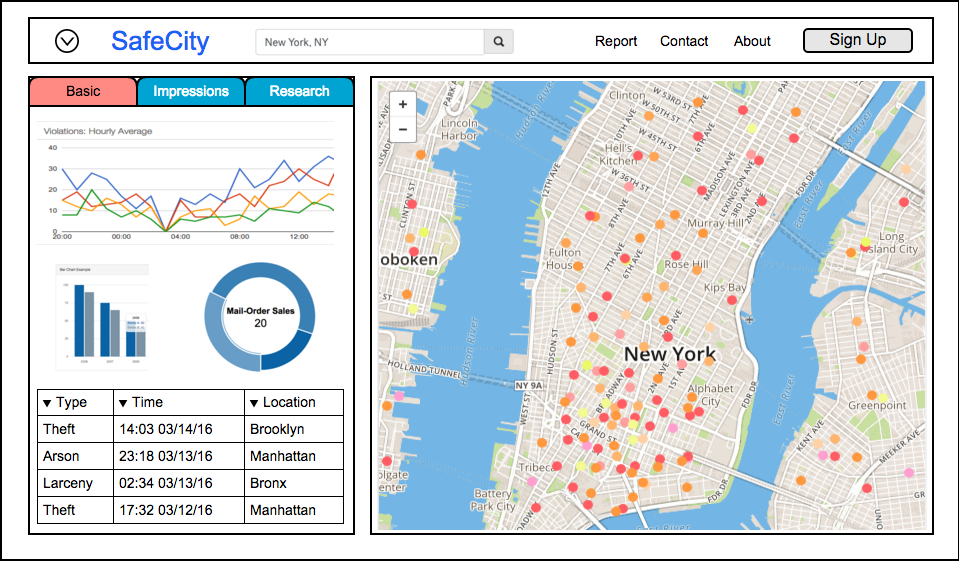
\includegraphics[width=10cm]{mockup}
\centering
\end{figure}

%------------------------------------------------

\subsection{Casual Passerby}

This user represents the people who stumble upon our site after having a transient interest in crime rates while surfing the web. The user will load the front page to find a large map taking up the rightmost two thirds of the screen, displaying all the crimes that happened in Manhattan in the last year as color coded bubbles. There will be a slider on the bottom of the map which will allow the user to play around with the time frame displayed on the map (maximum last ten years, minimum last week). The user can mouse over the map to find out details of each crime: time, type, and any people involved. To the left there will be a control panel summarizing the information in the map in different ways, which we hope will catch the user's eye for a few seconds. It will contain a line graph displaying the total number of crimes over time, a pie chart displaying all the different types of crimes, and a scrollable table containing all the crimes sorted chronologically. Once the user gets bored with Manhattan, he or she will type a different place, most likely his or her hometown, up in the search bar at the top of the screen and go through the same process and then leave.

%------------------------------------------------

\subsection{Active Member}

This user represents the people who have more lasting involvement with our application because they care about how the world views their community. This person will want the full benefits of being a member, so at some point they will click on the "Sign up" button on the top right and enter their username, password, full name, email address, and postal code (the last two will be verified). From then on they will either sign in through a login page or automatically sign in through their browser. This type of user has already explored the basic summaries mentioned above, and will spend more time on the second tab of the control panel: the impressions page. This page will be something like a Twitter feed, containing geotagged tweets involving safety or crime in an area, and containing a stack of 200 character testimonies people wrote about the safety of an area. Active members will be the primary contributors and curators of this information. They will write the testimonies about the areas in their city that they know, and they will upvote or downvote content as they feel fit to ensure that the most representative snippets are noticed. Periodically, these members will receive an email digest of what has been said about their area to invite them back.

%------------------------------------------------

\subsection{In-depth Researcher}

This user represents the people who are familiar to our site and come to it for more detailed and technical forms of information than those mentioned above. This user will occasionally check out the two tabs mentioned previously and be a member like the case above, but will spend most of their time viewing and downloading data from the third section of the control panel: the research tab. In this tab, the user will be able to download plain text files containing all the data used to make our application: all the times, types, and locations of crimes in an area and all the testimonials written about an area. The hope is that this user will use our information to gather further insights into how and why crime is happening. We will offer the option to upload documents in this tab, so that If the researcher uses our data to write a paper or report it can be made available to any other researchers looking to do something similar. Additionally, we will display our own take on using our data to research crime: a k-nearest-neighbors crime prediction algorithm which estimates the likelihood that certain crimes will happen in certain areas. This data will be overlaid to the right as a heatmap.

%----------------------------------------------------------------------------------------
% DESIGN
%----------------------------------------------------------------------------------------

\section{Design}

SafeCity will be implemented as a classic three-tier system, with the data tier (a MariaDB MySQL database with bash update scripts), logic tier (querying through PHP and Python preprocessing modules), and presentation tier (Bootstrap layout, KeenIO charts, and Google Maps API) will all be mutually independent. In general, the user will engage in a small action that prompts our business logic to request crime or user information from the database, which will be processed and then displayed for the user in a responsive format. \\

%------------------------------------------------

\subsection{Data}

This is a data driven application, so the data tier is arguably the most essential to its success. These days NoSQL databases like MongoDB are incredibly popular, but we have chosen to keep it simple with MariaDB relational database because we are certain our data will have a simple and uniform structure. There will be two tables: the first will store the type, time, longitude, and latitude of each crime; the second will store the name, username, password (md5 hashed), email, and zip code of each user. We will initialize the crime tables using data dumps of historical data, and then update them every day by scraping the webpages of different police and news stations with bash scripts that use wget or possibly BeautifulSoup. The users table will start out empty but every time a user signs up a row of information will be added. No values in the database will ever be deleted. We are not worried about running out of space because each entry in our databases takes only on the order of 10 bytes.

%------------------------------------------------

\subsection{Logic}

The role of the logic tier is to respond to requests from the presentation tier by retrieving information from the data tier and then process it before giving it to the presentation tier. A crime request will come as four floats: the minimum and maximum longitude and latitude of a rectangular area of the map. Using PHP select requests, we will query the database to find pull all crimes with longitude and latitude between the minimum and maximum (all the crimes in the area). It is not yet clear how we will make this operation quick when the amount of data we have gets very large, but for now we will likely allow the select operation to traverse all the crimes. Once these crimes are obtained, a python script will package them as a list of four-tuples (type, time, lattitude, longitude) and then send it to the presentation layer. A user request will come as a username and password pair. We will again use a PHP select statement to see if there are any users with that username and password and then return a pair to the presentation layer (username, zipcode) if the user exists and nothing otherwise. 

%------------------------------------------------

\subsection{Presentation}

The presentation tier is where the magic happens, our quick and intuitive way of presenting information will be an important differentiator from our competition. The overall layout will be a KeenIO template for an analytics dashboard, which we chose to keep the different sections organized. KeenIO is compatible with Bootstrap (in fact it was implemented with it), which will allow us to use Bootstrap's elegant buttons, search bar, and tables. Most importantly, both Bootstrap and KeenIO are responsive frameworks, so our website can be viewed on screens of different sizes (such as phone screens, our competitors cannot do this). Finally, the driver of the application is the map, which will be a Google Maps window displaying all the crimes given to it by the logic layer. Every time the user enters a new address, pans across the map, or selects a region of it, the maps API will return the center coordinates, length, and width of the current window (we think), which will then be sent to the logic layer in four tuple form for information retrieval.


%----------------------------------------------------------------------------------------
% TIMELINE
%----------------------------------------------------------------------------------------

\section{Timeline}

First, let us define certain landmarks which we shall be working towards in the coming weeks. \\

Prototype A: \\
This is the first checkpoint we will be working towards. Prototype A will have the infrastructure needed so that the app can access crime data and then work with the data in some way, either printing it out or populating a map with each crime. Prototype A will only have a map for New York City, but there will be options that categorize the crimes. For instance, you can select different options that show only crimes that happened in the past year, or in past years. \\

Prototype B: \\
The second checkpoint, Prototype B, will allow for a crime map of any area chosen by the viewer through an address and Google Maps. At this point, all data analytics for the app has been completed. Prototype B also includes a login and signup feature which will allow the user to create his or her own account for our application, as well as the impressions page. \\

Final product: \\
The final product will finally have the research tab. Moreover, all formatting and aesthetic decisions will be taken place here so the application looks clean and pleasing to the eye. \\

Now that we have defined three checkpoints. Here is the timeline for our project: \\

Week 1 (3/20-3/26): \\
Draw up on paper different layouts of our application and how the final product will look like.This will give us a good idea of what we?re working towards. \\
Setup the Github account for our project and make sure all logistics in that avenue are set up. \\
Project website as specified by the course website also will be built by 3/21 \\

Week 2 (3/27-4/3): \\
Build an application that takes in crime data and colors in a map with the individual entries. \\
This will be the prototype specified by the course website that is due this week. \\

Week 3 (4/4-4/10): \\
Categorization of crimes option should be finished by the end of this week. \\
By our standards, our Prototype A(lpha) should be done by this week itself.\\

Week 4 (4/11-4/17): \\
Demo Alpha version. 
Work on allowing any address or location to be populated with our data. 
Data analytics should be done at this point, so any remaining bugs should be fixed this week. \\

Week 5 (4/18-4/24): \\
Login and signup feature should be completed. \\
Impressions page completed \\

Week 6 (4/25-4/31): \\
Demo Beta version \\
Finish research tab \\
Work on aesthetics of application and fix any remaining bugs. \\

Week 7 (5/1-5/5): \\
Demo final product \\
Work on final documentation to be handed in on Dean?s Date \\

%----------------------------------------------------------------------------------------
% RISKS AND OUTCOMES
%----------------------------------------------------------------------------------------

\section{Risks and Outcomes}

When dealing with the publication and visualization of crime data, something that ultimately involves the safety of people?s lives, there will undoubtedly be many potential risks and outcomes that need to be carefully considered. \\

Our goal is to have data on crimes easily and widely available to anybody that decides to download our app. Searching for recent activity in a certain borough in New York City should immediately pull up all relevant crimes with additional details if desired. However, due to the negative nature of crimes, such information may trigger an over-exaggerated reaction to a situation that, in reality, needs context to understand properly. For example, a user looking for a place to travel may search up crime data on Queens, and if he or she finds a single entry on crime, might deem the area unsafe to visit. This is a completely natural and understandable reaction, but also biased. Is it possible for an area with a population of over two million people to be entirely devoid of crime? This bias will probably exist, and may skew local economics in unintended directions based upon misjudgements. However, our role as developers is to provide this data in an organized, but raw and unbiased form. The way the data is interpreted is out of our control. \\

In fact, we hope that the outcome of this project is exactly the aforementioned bias, but viewed in a more positive light. Our goal is not to discourage business in local stores or devalue houses in areas where crime rates are high, but to allow users to use their biases to make more informed judgements. If a user is extremely risk averse and will not tolerate a single crime in a certain area, well so be it, but at least he or she can use our app to easily make that judgement. Similarly, if a user doesn?t mind a few crimes per couple hundred thousand people, so be it as well, but once again, at least he or she can use our app to easily make that judgement. Our end goal is to quickly and effectively inform about crime, information that is important to the safety of the user. \\

\end{document}